\documentclass[a4paper]{ltxdoc}

\usepackage[UTF8]{ctex}
\usepackage{unicode-math}
\usepackage{caption}
\usepackage{booktabs}
\usepackage{xcolor}
\usepackage{listings}
\usepackage[perpage]{footmisc}
\usepackage{hypdoc}
\usepackage{amsfonts}
\usepackage{amsmath}
\usepackage{float}
\usepackage{graphicx}

\usepackage{geometry}
\geometry{left=3.3cm, right=3.3cm, top=2.5cm, bottom=3.0cm}

\usepackage{color}

\makeatletter

% 设置字体
\IfFileExists{/System/Library/Fonts/Times.ttc}{
  \setmainfont{Times}
  \setsansfont[Scale=MatchLowercase]{Helvetica}
  \setmonofont[Scale=MatchLowercase]{Menlo}
  \xeCJKsetwidth{‘’“”}{1em}
}{}
\unimathsetup{
  math-style=ISO,
  bold-style=ISO,
}
\IfFontExistsTF{xits-math.otf}{
  \setmathfont[
    Extension    = .otf,
    BoldFont     = *bold,
    StylisticSet = 8,
  ]{xits-math}
  \setmathfont[range={cal,bfcal},StylisticSet=1]{xits-math.otf}
}{
  \setmathfont[
    Extension    = .otf,
    BoldFont     = XITSMath-Bold,
    StylisticSet = 8,
  ]{XITSMath-Regular}
  \setmathfont[range={cal,bfcal},StylisticSet=1]{XITSMath-Regular.otf}
}

% 定义一些命令用于写文档
\newcommand\TeXLive{\TeX{} Live}
\newcommand\unicodechar[1]{U+#1(\symbol{"#1})}
\DeclareRobustCommand\file{\nolinkurl}
\DeclareRobustCommand\env{\texttt}
\DeclareRobustCommand\pkg{\textsf}
\DeclareRobustCommand\cls{\textsf}
\DeclareRobustCommand\opt{\texttt}

% 在 doc 的基础上增加 option 的描述
\def\DescribeOption{\leavevmode\@bsphack\begingroup\MakePrivateLetters
  \Describe@Option}
\def\Describe@Option#1{\endgroup
              \marginpar{\raggedleft\PrintDescribeOption{#1}}%
              \SpecialEnvIndex{#1}\@esphack\ignorespaces}
\@ifundefined{PrintDescribeOption}
   {\def\PrintDescribeOption#1{\strut \MacroFont #1\ }}{}

% 调整列表的格式
\setlength\partopsep{\z@}
\def\@listi{\leftmargin\leftmargini
            \parsep \z@
            \topsep \z@
            \itemsep \z@}
\let\@listI\@listi
\@listi

% listings 的样式
\lstdefinestyle{lstshell}{
  basicstyle      = \small\ttfamily,
  backgroundcolor = \color{lightgray},
  language        = bash,
}
\newcommand\shellcmd[1]{\colorbox{lightgray}{\lstinline[style=lstshell]|#1|}}
\lstnewenvironment{shell}{\lstset{style=lstshell, gobble=2}}{}
\lstnewenvironment{latex}{%
  \lstset{
    basicstyle = \small\ttfamily,
    frame      = single,
    gobble     = 2,
    language   = [LaTeX]TeX,
  }%
}{}

\hypersetup{
  allcolors         = blue,
  bookmarksnumbered = true,
  bookmarksopen     = true,
}
\makeatother


\begin{document}



\title{Matlab-1}
\author{高悟恒 }
\date{\qquad 2020-09-17}
\maketitle



一.算法:
设有给定插值条件:起点$x_i(p_i),i=1,...,n$和终点$q_i,i=1,..,n$。\\
1.IDW:\\
取形式为$f(x)=\sum_{i=1}^n \omega_i f_i(x)$的函数作为插值函数。\\
其中$f_i(x)=q_i+D_i(x-p_i)$,根据论文这里选取$D_i$为线性变换。\\
因此$D_i$为一个二阶方阵,记为$(d_{i,kl}),k,l=1,2$。\\
由$D$导致的误差函数为:$E_i(D)=\sum_{j=1,j\neq i}^n \omega_{ij}\parallel q_i+D(x_j-x_i)-q_j\parallel^2=\sum_{j=1,j\neq i}^n \omega_{ij}((d_{11}(p_{j,1}-p_{i,1})+d_{12}(p_{j,2}-p_{i,2})+q_{i,1}-q_{j,1})^2+(d_{21}(p_{j,1}-p_{i,1})+d_{22}(p_{j,2}-p_{i,2})+q_{i,2}-q_{j,2})^2$。\\
其中系数$\omega_{ij}$应当由$x_i$和$x_j$的距离决定,一种简单有效的选择是$\omega_{ij}=\sigma_i(x_j),\sigma_i(x)={1\over (d_i(x))^\mu}$。\\
求误差函数最小值是一个极小二乘问题,只需对$d_{kl}$求偏导取零即可。\\
权重函数$\omega_i$需满足条件$\omega_i(x)\geq 0,\sum_{i=1}^n\omega_i(x)=1,\omega_i(x_j)=\delta_{ij}$。\\
论文中选取了$\omega_i(x)={\sigma_i(x) \over\sum_{i=1}^n\sigma_j(x)},\sigma_i(x)={1\over (d_i(x))^\mu},\mu>0$,这里为了便于计算通常选取$\mu=2$。\\
2.RBF:\\
取形式为$T(x)=A(x)+R(x)$的函数作为插值函数。\\
其中$A(x)=Mx+b$为仿射变换,可以根据初始设定计算,这里我们选取其为恒等变换。\\
而$R(x)$为径向基函数,$R(x)=\sum_{i=1}^n a_i g(||x-x_i||)$,这里选取$g(d)=(d^2+r^2)^{\mu/2},\mu=-1$,其中$r_i=\min{\{i\neq j\}}d(x_i,x_j)$。\\
最后参数$a_i$可以由给定的插值条件求解方程组得到。\\


\newpage
二.实验结果:
\begin{figure}[htb]
  \centering
  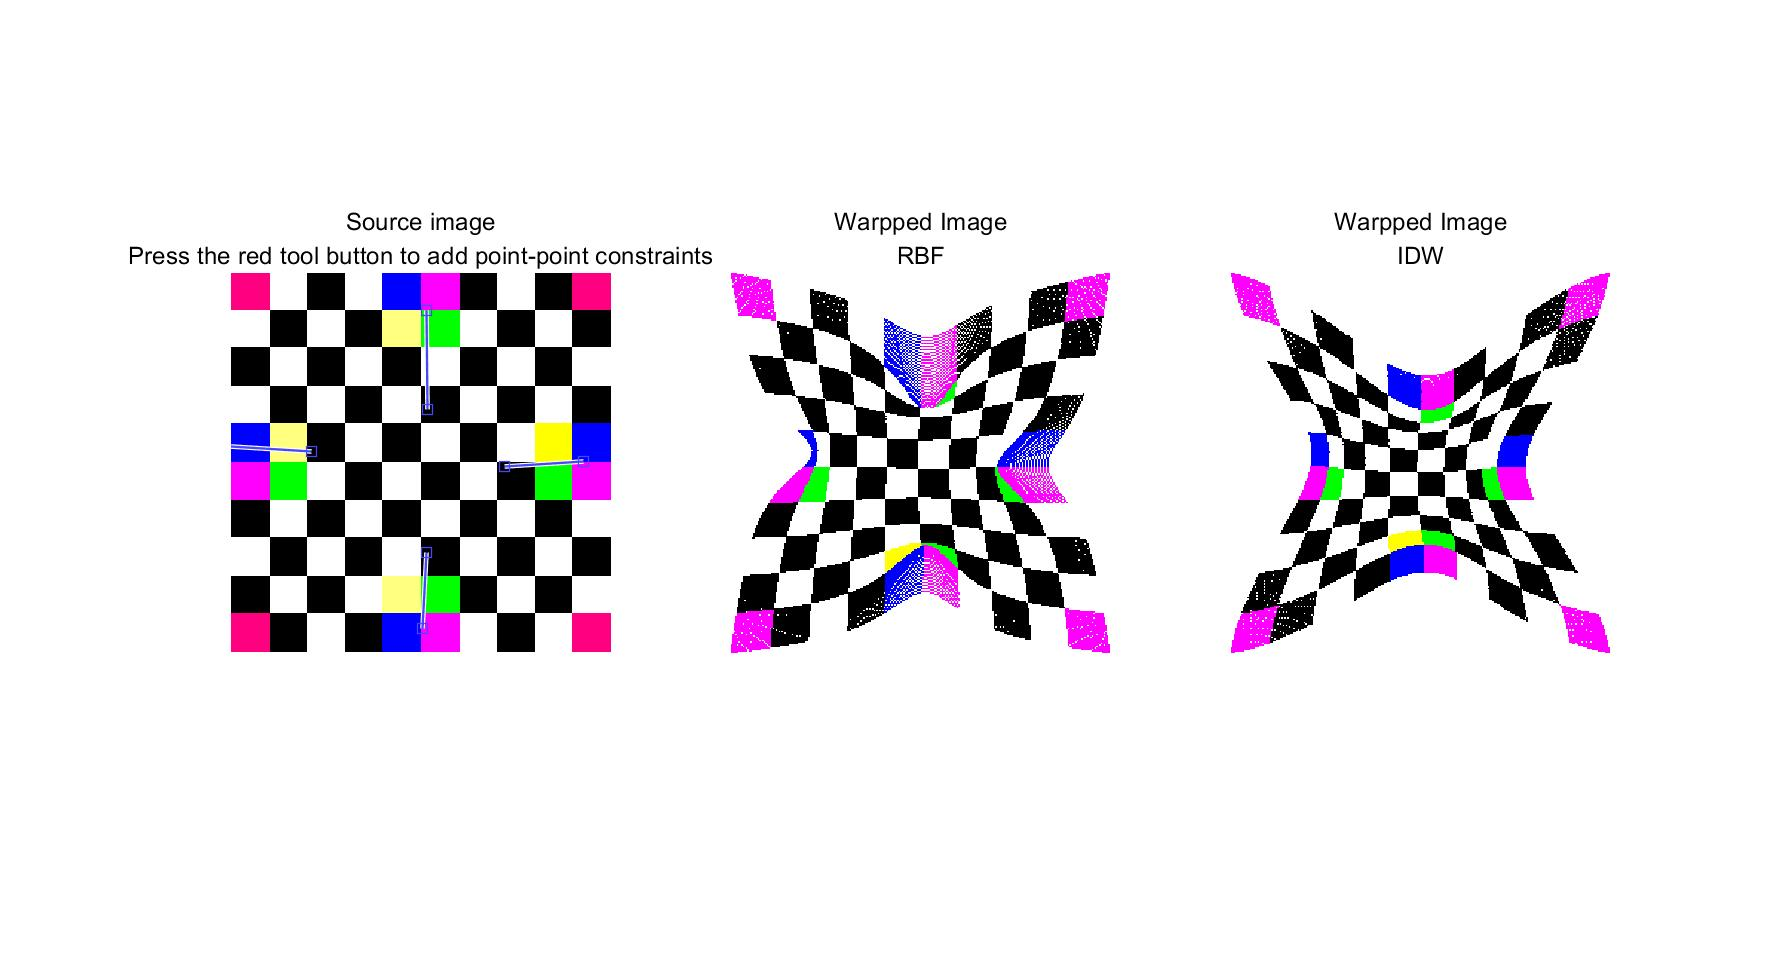
\includegraphics[width=1.0\textwidth]{fig1.jpg}
  \caption{变形效果(压缩)}
  \label{fig:fig-1}
%  \note{注:这里固定四个角,压缩四条边的中点处}
\end{figure}

\begin{figure}[htb]
  \centering
  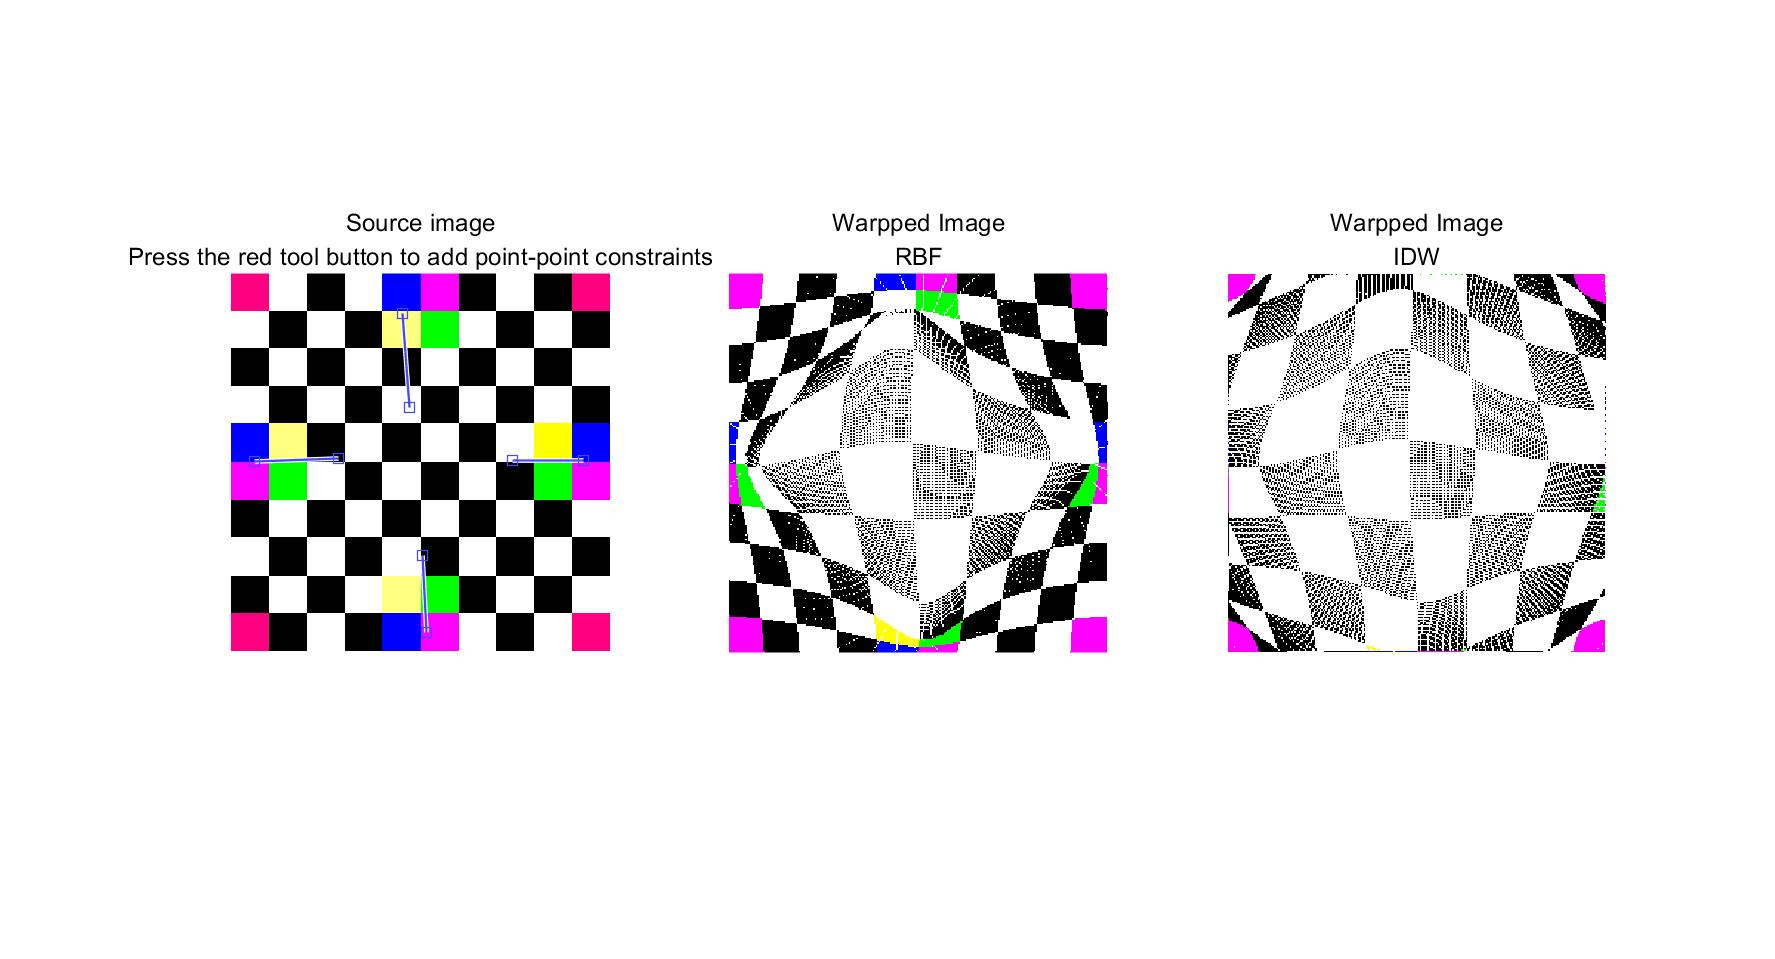
\includegraphics[width=1.0\textwidth]{fig2.jpg}
  \caption{变形效果(拉伸)}
  \label{fig:fig-1}
%  \note{注:这里固定四个角,拉伸四条边的中点处}
\end{figure}

\newpage
这里我们首先固定住四个角,再分别压缩或拉伸四条边的中点处,可以看到两种方法的计算效果都较好,但是值得注意的是变换后的图片中有一些白缝。

三.白缝:
这两种方法都是寻找一种连续的插值函数对图像进行变换,但是图像本身是离散的,这就导致我们只能计算原有图像上的点对应的点,而为了得到新的图像就需要对计算出来的点进行取整。又由于函数必然不是线性的,因此就会出现原来密集的点映射到相对较分散的区域的情况,这就产生了白缝。
















*****************************************************************\\
\end{document}
